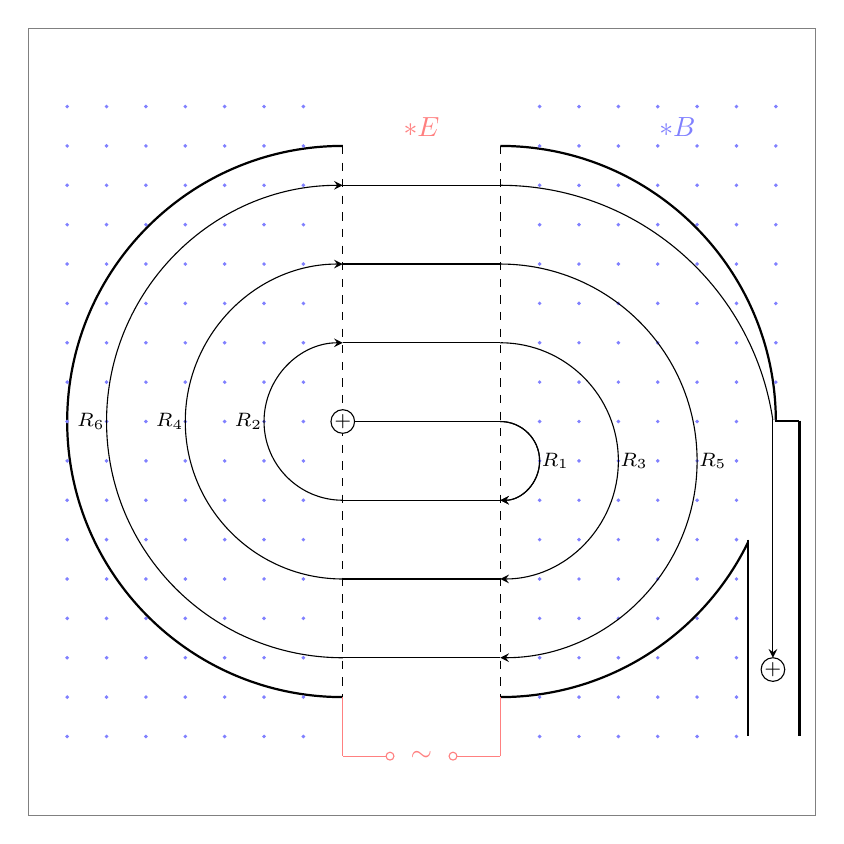
\begin{tikzpicture}[scale=1]
    \draw[gray,ultra thin] (-5,-5) rectangle (5,5);

    \draw[dashed,thin] (-1,3.5)--(-1,-3.5);
    \draw[dashed,thin] (+1,3.5)--(+1,-3.5);
    \draw[thick] (+1,3.5) arc (90:-90:3.5);
    \draw[thick] (-1,3.5) arc (90:270:3.5);

    \foreach \x in {-4.50,-4.00,...,-1.50}
    {
        \foreach \y in {-4.00,-3.50,...,4.00}
        {
            \fill[blue!50!white] (\x,\y) circle (0.025);
        }
    }
    \foreach \x in {+4.50,+4.00,...,+1.50}
    {
        \foreach \y in {-4.00,-3.50,...,4.00}
        {
            \fill[blue!50!white] (\x,\y) circle (0.025);
        }
    }
    
    \draw[-stealth] (1,0) arc (90:-90:0.5);

    \foreach \y in {0,1,2,3}
    {
        \draw (-1,\y)--(1,\y);
    }

    \foreach \y in {-1,-2,-3}
    {
        \draw (1,\y)--(-1,\y);
    }

    \begin{scope}
        \clip (+1,0) circle (3.5);
        \foreach \y in {0,1,2,3}
        {
            \draw[-stealth] (1,\y) arc (90:-90:\fpeval{\y+0.5});
            \node[right] at (\fpeval{\y+1.5-0.1},-0.5) {\scriptsize $R_{\fpeval{2*\y+1}}$};
        }
    \end{scope}

    \begin{scope}
        \foreach \y in {-1,-2,-3}
        {
            \draw[-stealth] (-1,\y) arc (-90:-270:\fpeval{-\y});
            \node[left] at (\fpeval{\y-1+0.1},0) {\scriptsize $R_{\fpeval{-\y*2}}$};
        }
    \end{scope}

    \fill[white] (4.15,0.02) rectangle (4.6,-4.9);
    \draw[thick] (4.485,0.01)--(4.8,0.01);
    \draw[thick] (4.8,0.01)--(4.8,-4);
    \draw[thick] (4.15,-1.5)--(4.15,-4);
    \draw[-stealth] (4.463,0.022)--(4.463,-3);

    \draw[fill=white] (-1,0) circle (0.15) node {\scriptsize $+$};
    \draw[fill=white] (4.463,-3.15) circle (0.15) node {\scriptsize $+$};

    \node[above,red!50!white] at (0,3.5) {$\vb*{E}$};
    \node[above,blue!50!white] at (3.25,3.5) {$\vb*{B}$};

    \draw[red!50!white] (-1,-3.5)--(-1,-4.25);
    \draw[red!50!white] (+1,-3.5)--(+1,-4.25);
    \draw[red!50!white] (+1,-4.25)--(+0.4,-4.25);
    \draw[red!50!white] (-1,-4.25)--(-0.4,-4.25);
    \draw[red!50!white,fill=white] (-0.4,-4.25) circle (0.05);
    \draw[red!50!white,fill=white] (+0.4,-4.25) circle (0.05);
    \node[red!50!white] at (0,-4.25) {$\sim$};
\end{tikzpicture}
